Considera la funció
\[
f(x)=-x^3+6x^2-9x+4 .
\]

\begin{apartats}

\apartat[1,25]{1}
Troba'n els punts de tall amb els eixos, estudia'n la monotonia i troba'n els extrems
relatius.

\begin{solucio}
\textbf{Talls}: $f(0)=4$, el punt $(0,4)$. Per a l'eix $OX$, $x=1$ és arrel ($f(1)=-1+6-9+4=0$) i,
dividint, $f(x)=-(x-1)^2(x-4)$: els talls són $(1,0)$, amb arrel doble, i $(4,0)$.\\
\textbf{Monotonia}: $f'(x)=-3x^2+12x-9=-3(x-1)(x-3)$, que s'anul·la en $x=1$ i $x=3$.\\
$f$ \textbf{decreix} a $(-\infty,1)$, \textbf{creix} a $(1,3)$ i \textbf{decreix} a $(3,+\infty)$.\\
\textbf{Mínim relatiu} $(1,0)$ i \textbf{màxim relatiu} $(3,4)$.
\end{solucio}

\begin{nomesllarg}
\apartat{0,75}
Estudia'n la curvatura i troba'n el punt d'inflexió.

\begin{solucio}
$f''(x)=-6x+12$, que s'anul·la en $x=2$.\\
$f''>0$ a $(-\infty,2)$: \textbf{convexa}. \quad $f''<0$ a $(2,+\infty)$: \textbf{còncava}.\\
Com que la curvatura hi canvia i $f(2)=2$, el punt d'inflexió és $(2,2)$.
\end{solucio}
\end{nomesllarg}

\begin{tria}{estudi-tasca}
\itemtria{original}{0,75}{1,25}
Representa la funció amb tota la informació anterior.

\begin{solucio}
La gràfica ve de $+\infty$, baixa fins a tocar l'eix en el mínim $(1,0)$, puja fins al màxim $(3,4)$ i
baixa cap a $-\infty$, tallant l'eix en $(4,0)$. Com que el coeficient de $x^3$ és negatiu, les
branques van al revés que les de $x^3$.
\begin{center}
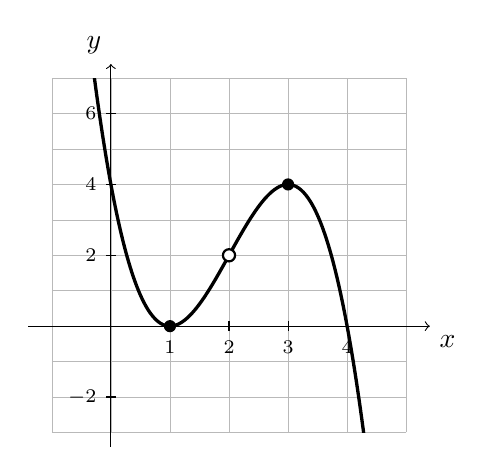
\begin{tikzpicture}[x=0.75cm,y=0.45cm]
  \draw[gray!55,very thin,step=1] (-1,-3) grid (5,7);
  \draw[->] (-1.4,0) -- (5.4,0) node[below right] {$x$};
  \draw[->] (0,-3.4) -- (0,7.4) node[above left] {$y$};
  \foreach \i in {1,2,3,4} \draw (\i,0.15) -- (\i,-0.15) node[below,font=\scriptsize] {$\i$};
  \foreach \j in {-2,2,4,6} \draw (0.08,\j) -- (-0.08,\j) node[left,font=\scriptsize] {$\j$};
  \begin{scope}
    \clip (-1,-3) rectangle (5,7);
    \draw[\colorgrafica,very thick,domain=-0.4:4.5,samples=120,smooth] plot (\x,{-(\x)*(\x)*(\x)+6*(\x)*(\x)-9*(\x)+4});
  \end{scope}
  \fill (1,0) circle (2.2pt); \fill (3,4) circle (2.2pt);
  \draw[fill=white,thick] (2,2) circle (2.2pt);
\end{tikzpicture}
\end{center}
\end{solucio}

\itemtria{tangent-inflexio}{0,75}{1,25}
Troba la recta tangent a la gràfica en el punt d'inflexió, i digues a quina banda de la tangent
queda la gràfica a cada costat d'aquest punt.

\begin{solucio}
$f''(x)=-6x+12$ s'anul·la i canvia de signe en $x=2$, i $f(2)=2$: el punt d'inflexió és $(2,2)$.\\
$f'(2)=-12+24-9=3$, i la tangent és $y=2+3(x-2)$, és a dir $\boxed{y=3x-4}$.\\
$f(x)-(3x-4)=-x^3+6x^2-12x+8=-(x-2)^3$, que és positiu si $x<2$ i negatiu si $x>2$. La gràfica queda
\textbf{per sobre} de la tangent a l'esquerra i \textbf{per sota} a la dreta: en un punt d'inflexió,
la corba \textbf{travessa} la tangent.
\end{solucio}
\end{tria}

\end{apartats}
